% Reset counters and commands for appendix
\setcounter{chapter}{0}
\renewcommand{\thechapter}{\Alph{chapter}}
\setcounter{equation}{0}
\renewcommand{\theequation}{\Alph{chapter}.\arabic{equation}}
\setcounter{figure}{0}
\renewcommand{\thefigure}{\Alph{chapter}.\arabic{figure}}
\setcounter{table}{0}
\renewcommand{\thetable}{\Alph{chapter}.\arabic{table}}
\appendix
\chapter{Macでの研究環境の構築}
ここでは、Macで研究環境を構築する祭に最低限やるべきこと、知っておくべきことを説明します。Macに限らずWindowsやLinuxでも、計算機環境の設定は個々人の好みや研究内容によって大きく変わります。そのため、ここに書くことは参考程度にとどめて下さい。
\section{英語環境にする}
日本の研究室でMacを使う場合、OSの言語環境を日本語にしている人が多いでしょう。しかしMacを研究で使う場合には英語環境に変更することを強くお勧めします。大きく四つの理由があるからです。

まず第一に、インターネット上のMac関係の情報の多くが英語で書かれており、英語で検索した場合に見つかる情報の量と質は日本語の情報を圧倒するからです。使っているMacで何か問題が生じた場合にエラーメッセージが日本語で表示されていると、それを検索語にしても辿り着ける情報には限りがあります\footnote{\LaTeX 関係などの情報だと日本語特有の問題も発生しうるので、そこは臨機応変に対応して下さい。}。Apple社はアメリカの企業でありMacユーザの多くが北米に集中しています。そのためMac関連の情報のやり取りの多くは英語でなされています。これはMacに限らずコンピュータ関係全般に言えます\footnote{恐らく唯一の例外がRubyというプログラミング言語です。これは日本人により開発されたものが世界に広がった希有な例です。}

第二に、あなたは日本人のみと共同研究をするわけではないからです。もしあなたのMacの画面を外国人が見ながら、もしくはあなたが外国人のMacの画面を見ながら作業する時に、OSが英語環境になっていたほうが意志疎通が簡単になることは言うまでもないでしょう。また海外(特にアメリカ)の研究機関などで実験をするときに、現地で使用するMacが英語環境になっているのは当然です。

第三の理由は、ファイル名やメニューの表示が英語になっているほうが作業効率が上がるからです。Macだとホームディレクトリに「書類」や「デスクトップ」というディレクトリが存在しますが、英語環境ではそれぞれ「Documents」と「Desktop」です。Terminal.appからホームで\texttt{ls}すれば、実体が英語名だということがわかります。Finder.appからディレクトリの移動をしたいときに、英語環境であればホームを開いた状態で「do」と連打すれば「Documents」が選択された状態になります。また「de」と打てば「Desktop」が選択されます。日本語環境の場合にはこのようにはいきません。またメニューの「編集」は英語環境では「Edit」になっています。メニューで「Edit」を開いた状態で「co」と連打すれば「Copy」のところが選択された状態になるでしょう。

最後の理由は、できる限り英語に慣れ親しんだほうが良いからです。大学院に入りたての頃は、誰しも英語の読み書きと会話に苦労するでしょう。また日本人の多くの研究者はその後何十年も英語で苦労をし続けます。少しでも英語に慣れるため、常用するMacくらい英語環境で使う意志を持ちましょう。

ただし、英語環境にすることで問題が生じる場合があります。例えば英語環境でFLASHを表示すると日本語が文字化けすることがあります。これはFLASHが既に廃れつつある技術であり、かつFLASHの開発チームが能力不足だからです。他にも英語環境にすると日本語表示がうまくいかないソフトがあるかもしれませんが、そのようなソフトを使うのはやめましょう。日本語表示以外にも色々と問題を抱えている可能性があります。

図\ref{fig_English1_png}から図\ref{fig_English3_png}のように「システム環境設定」から英語環境に変更することができます。この設定後に起動したアプリケーションは、全て英語環境として起動されます。全てのメニューなどが英語で表示されるはずです。図\ref{fig_English3_png}にある「単語区切り」の設定は忘れないようにして下さい。ダブルクリックで日本語文字列を選択する場合に、熟語やカタカナ語が一つの単語として認識されるようになります。

\begin{figure}
  \begin{center}
    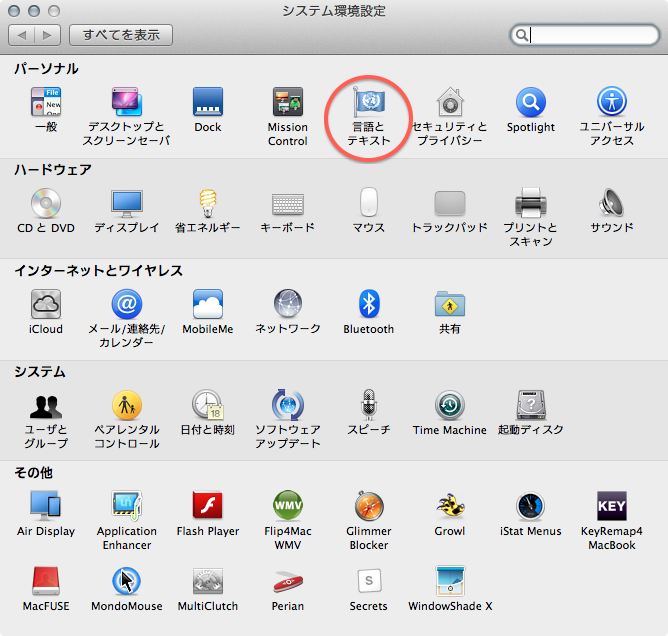
\includegraphics[scale=0.4,bb= 0 0 668 636]{fig/English1.png}
    \caption{「システム環境設定」から「言語とテキスト」を開く}
    \label{fig_English1_png}
  \end{center}
\end{figure}

\begin{figure}
  \begin{center}
    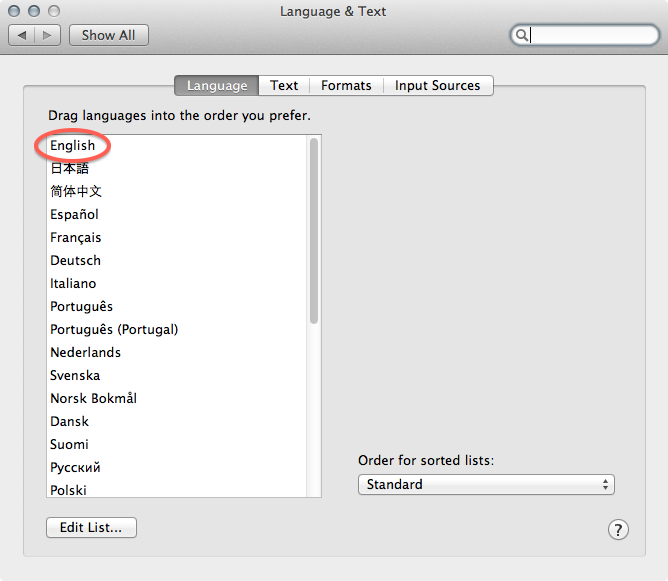
\includegraphics[scale=0.4,bb= 0 0 668 636]{fig/English2.png}
    \caption{「日本語」ではなく「English」を先頭に持ってくる(この画面は既に英語環境になっている場合のもの)}
    \label{fig_English2_png}
  \end{center}
\end{figure}

\begin{figure}
  \begin{center}
    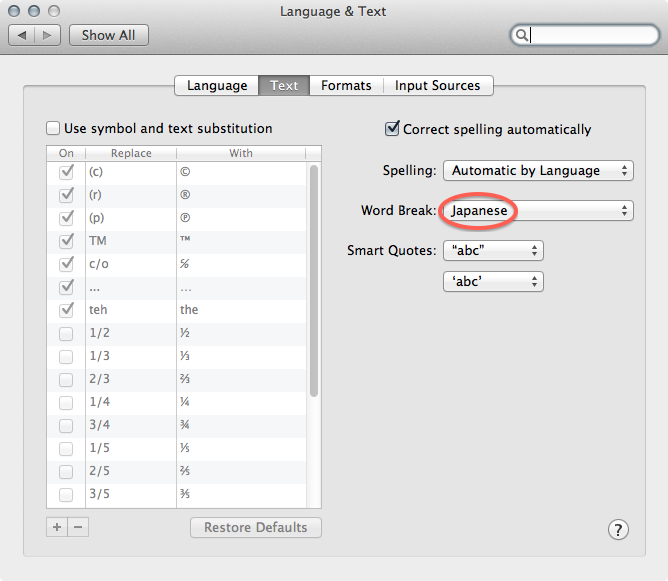
\includegraphics[scale=0.4,bb= 0 0 668 636]{fig/English3.png}
    \caption{「単語区切り(Word Break)」を「Japanese」にする(この画面は既に英語環境になっている場合のもの)}
    \label{fig_English3_png}
  \end{center}
\end{figure}


\section{拡張子を表示する}
Macの初期設定では、ファイルの拡張子(extension)が表示されません。図~\ref{fig_Extension_png}のようにFinder.appの「Preferences\ldots」から表示する設定に変更しましょう。この表示をしないと、Terminal.appから操作するファイル名とFinder.appからファイル名が見かけ上一致しない場合があります。

\begin{figure}
  \begin{center}
    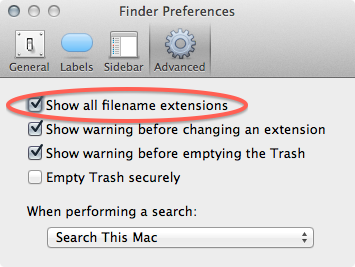
\includegraphics[scale=0.4,bb= 0 0 355 267]{fig/Extension.png}
    \caption{「単語区切り(Word Break)」を「Japanese」にする(この画面は既に英語環境になっている場合のもの)}
    \label{fig_Extension_png}
  \end{center}
\end{figure}

\section{キーボードの設定}

もしあなたのMacがUS配列のキーボードならば、Caps LockキーはControlキーとして機能するように設定を変更しましょう。図\ref{fig_Keyboard1_png}のように、System Preferencesから「Keyboard」を開き、Caps LockをControlにします。また、「Keyboard Shortcuts」のタブに移動し、ボタンなどの選択を全てtabキーで行えるようにします。このようにすることで、様々な画面操作をするときに、いちいちキーボードからトラックパッドやマウスへ手の移動をしなくて済むようになります。

\begin{figure}
  \begin{center}
    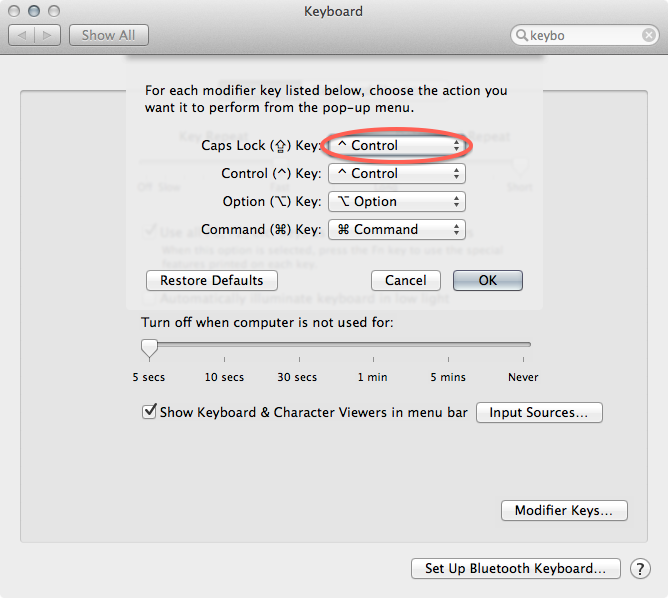
\includegraphics[scale=0.4,bb= 0 0 668 636]{fig/Keyboard1.png}
    \caption{Caps LockをCntrolキーに変更する}
    \label{fig_Keyboard1_png}
  \end{center}
\end{figure}

\begin{figure}
  \begin{center}
    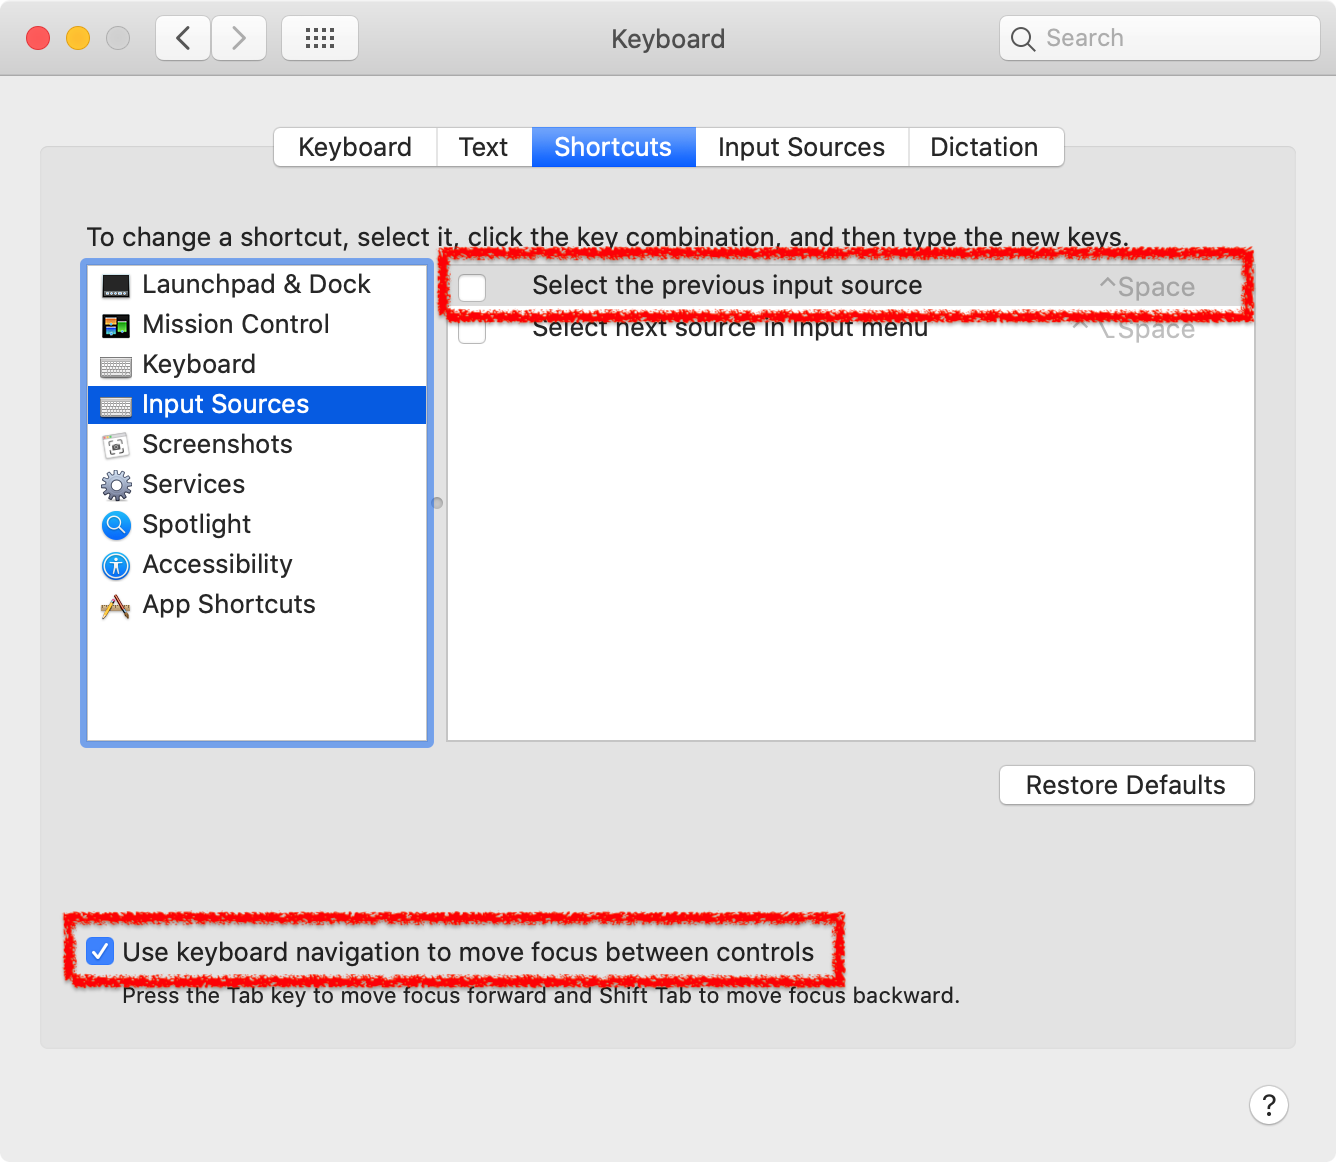
\includegraphics[scale=0.4,bb= 0 0 668 636]{fig/Keyboard2.png}
    \caption{全てのボタンなどをtabキーで移動できるようにする}
    \label{fig_Keyboard2_png}
  \end{center}
\end{figure}

\section{Xcode}
\section{KeyRemap4MacBook}
\section{zsh}
\section{MacPorts}
\subsection{Emacs}
\subsection{\LaTeX}

